\documentclass[slides]{pgnotes}

\title{DataBase Management Systems (DBMS)}

\begin{document}

\maketitle

\tableofcontents

\section{Database management systems (DBMS)}\label{sec:dbms}

DataBase Management Systems (DBMS) persistently store data records according to a schema.

\begin{bluebox}{Key concepts}
\begin{description}
\item[Schema] defines \textit{how} data is stored. Defines rules.
\item[Records] of logically grouped data (e.g. a customer, an invoice)
\end{description}
\end{bluebox}

\subsection{Required functionality}

\begin{greenbox}{Must provide}
\begin{description}
\item[Data storage/retrieval:] fundamental reason for using! 
\item[Catalog] of schema and data stored
\item[Transaction support] for batch updates to be applied atomically
\item[Concurrency control] to manage simultaneously connected clients
\item[Recovery] to a working state after hardware / software failures
\item[Authorization services] to verify connected clients identity and control access.
\item[Data communication support] to allow usage from remote computers.
\item[Integrity services] to enforce constraints on data as defined by the user.
\end{description}
\end{greenbox}

\subsection{Families}

\begin{greenbox}{Relational databases}
  \begin{itemize}
  \item Sometimes called \textbf{SQL databases}.
  \item Examples: Oracle, PostgreSQL, MySQL, Microsoft SQL.
  \end{itemize}
\end{greenbox}

\begin{bluebox}{Non-relational databases}
  \begin{description}
  \item[Key-Value stores] that associate a key with a value. (e.g. Redis)
    \begin{itemize}
    \item Optimised for fast lookup of small pieces of data
    \end{itemize}
  \item[Document databases] that store a semi-structured document identified by a key (e.g. MongoDB)
    \begin{itemize}
    \item Useful for semi-structured data accessed as a whole
    \end{itemize}
  \item[Graph databases] that store nodes and their relationships (e.g. Neo4J)
    \begin{itemize}
    \item Mapping, transport planning, relationships, likes, friends.
    \end{itemize}
  \end{description}
\end{bluebox}

We'll begin on \textbf{relational databases} using \textbf{PostgreSQL}.




\subsection{Text-based query language}

Most database systems incorporate a native programming language allowing us either directly or via a client application manipulate the database: 

\begin{greenbox}{3 roles:}
\begin{description}
\item[Data Definition (DDL)] to work with schema.
\item[Data Manipulation (DML)] to work with data stored according to the schema.
\item[Query language] for accessing data
\end{description}
\end{greenbox}

Usually a common language provides all of these functions.
SQL best known:

\begin{minted}{sql}
  SELECT name, finish_time
  FROM competitors
  ORDER BY finish_time DESC;
\end{minted}

\subsection{Database host}

The server process manages the data store and processes requests from clients.
The server can be running on any of the following \emph{hosts}:

\begin{greenbox}{Hosts}
  \begin{itemize}
  \item
    Standard laptop / desktop computer
  \item
    Dedicated server computer (in a data centre environment)
  \item
    Cloud-based virtual host, called a compute instance. (e.g.~Amazon EC2)
  \item
    A managed database service provided by a cloud service provider
    (e.g.~Amazon RDS, Azure, Google Cloud, IBM Cloud)
  \end{itemize}
\end{greenbox}

Database is often a critical piece of our infrastructure and needs to be provisioned appropriately. \textit{Will discuss data centre environment later on!}

DBMS can run on a variety of Operating Systems (often UNIX / Linux):
\begin{itemize}
\item We will learn how to use PostgreSQL within a Unix (Linux) environment.
\end{itemize}



\subsection{Client-server}\label{client-server}

Most database management systems run in a client-server model, even on the same host.

\begin{figure}[htbp]
  \centering
  \includegraphics[width=0.7\linewidth]{dbms_client_server}
  \caption{Client-Server model}
  \label{fig:client-server-model}
\end{figure}


\subsection{Protocol}

The client program accesses the server using a server-specific protocol.

Clients normally access the server through IP networks using TCP on a specified port number.

\begin{greenbox}{Examples of clients}
\begin{itemize}
\item
  Most databases have a simple command-line client that can send
  requests to the database and display results
\item
  Apps can be written to access database servers using a client library.

  \begin{itemize}
  
  \item
    Generally the text-mode client uses this library internally too!
  \end{itemize}
\end{itemize}
\end{greenbox}

\begin{redbox}{Important note about clients}
\begin{itemize}
\item
  The client may in some cases be running on the same host as the
  server.
\item
  Software that is the client of a DBMS may itself be a server of another type.
\end{itemize}
\end{redbox}



\subsection{Concurrency}
\label{sec:concurrency}

This also implies that there is a degree of concurrency, where multiple
clients access the same database at the same time.

\begin{figure}[htbp]
  \centering
  \includegraphics[width=1.0\linewidth]{dbms_concurrent_access}
  \caption{Concurrent access to a college timetable database}
  \label{fig:concurrent-access}
\end{figure}

Clients are often heterogeneous, where different types of clients concurrently access the same data.



\subsection{Remote access}

A particular pattern you will encounter is where the client program runs on the same host as the DBMS, and remote shell access is used to permit clients to connect to the server.

\begin{figure}[htbp]
  \centering
  \includegraphics[width=1.0\linewidth]{ssh_psql_usage}
  \caption{SSH access to a remote database}
  \label{fig:ssh-psql-usage}
\end{figure}





\section{PostgreSQL}\label{sec:postgresql}

We will focus on PostgreSQL as our primary database.


\begin{greenbox}{Reasons for choice of PostgreSQL:}
\begin{itemize}
\item
  It is free software
\item
  Can be installed on many operating systems.
\item
  No limits / free-trial limitations.
\item
  Support exists for geospatial data, JSON, XML, full-text search etc.
\item
  Has some support for masquerading as other types of DB (e.g. graph data).
\item
  High adoption among many analytics and data science workloads.
\end{itemize}
\end{greenbox}

As we continue we will refer to PostgreSQL as \textbf{Postgres} for brevity.

On a single host, a relational database management system \textbf{cluster} provides one or more isolated \textbf{databases}.
Within a database, data is contained in one or more \textbf{tables} according to the \textbf{schema}.


\section{Defining characteristics}

Codd's Seminal paper defines a set of characteristics that a relational database must possess.

We'll use these to explore the basic anatomy of a relational database, specifically PostgreSQL.

Note: the order of these rules has been adjusted to introduce some concepts in a more logical way!


\subsection{Foundation rule}

\textbf{For any system that is advertised as, or claimed to be, a relational database management system, that system must be able to manage databases entirely through its relational capabilities.}
  
\subsection{Information Rule}
  
\textbf{All information in a relational database is represented explicitly at the logical level and in exactly one way --- by values in tables.}

\subsubsection{Relational data structure}

\begin{figure}[htbp]
  \centering
  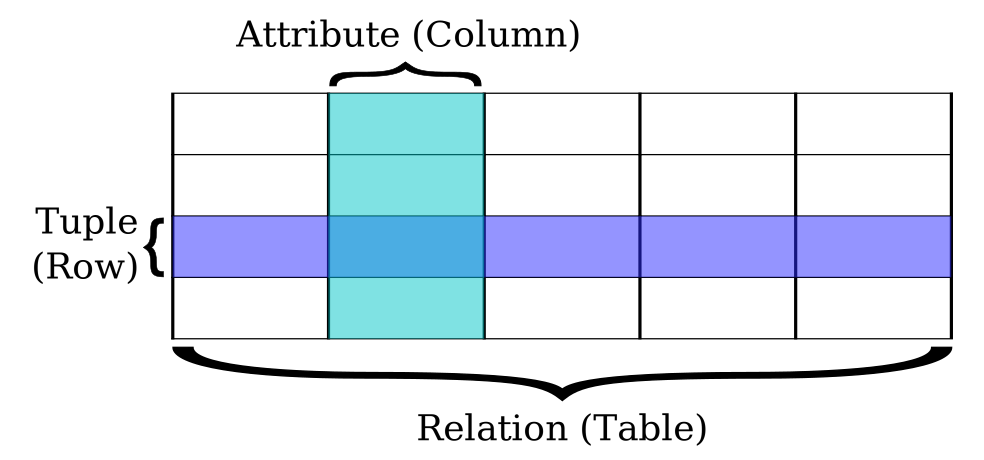
\includegraphics[width=0.5\linewidth]{rdbms_terms}
  \caption{Relational model terminology}
  \label{fig:rdbms-terms}
\end{figure}

\begin{description}
\item[Relation (Table):] with columns and rows. Table names must be unique.
  \begin{description}
  \item[Base relation] is a table defined in the database schema
  \item[Derived relation] is a virtual table that appears in response to a query
  \end{description}
\item[Attribute (Column):] holding distinct part of a row: 
  \begin{itemize}
  \item Column names must be unique within a table.
  \item Column has a \textbf{data type} (e.g. integer, text) from an allowable list (database-dependent).
  \item Column may allow / permit \textbf{null} values (unknown, empty, undefined, blank)
  \item Column order has no meaning or significance.
  \end{itemize}
\item[Tuple (Row):] a single record contained with a table.
  \begin{itemize}
  \item No theoretical upper limit on number of rows.
  \item The natural order of rows in a table is meaningless!  Do not rely on it!
  \end{itemize}
\end{description}

\subsection{Systematic treatment of null values}
  \textbf{Null values (distinct from the empty character string or a string of blank characters and distinct from zero or any other number) are supported in fully relational DBMS for representing missing information and inapplicable information in a systematic way, independent of data type.}

\subsubsection{Null}

Null denotes a lack of a value, used to indicate that data is missing, unknown, blank, undefined:
\begin{itemize}
\item Null is \textbf{not} zero, the empty string, false or any other value.
\item Null values will \textbf{pollute other expressions} (e.g. arithmetic, comparison)
  \begin{itemize}
  \item Null does not even equal null!
  \end{itemize}
\item \textbf{Can test} for null with \texttt{IS NULL} operation.
\end{itemize}
While the concept of null can be confusing, it avoids placeholder data.



\subsection{Integrity independence}

\textbf{Integrity constraints specific to a particular relational database must be definable in the relational data sublanguage and storable in the catalog, not in the application programs.}

\subsubsection{Unique constraint}

Within a table, a unique constraint on a column or group of columns will prevent duplicate rows existing.  

\newpage

\subsubsection{Primary key}

Practically we need ways to identify any row individually.
Within any table, there may be a number of \textbf{candidate keys} that could be used to identify each row.
\begin{description}
\item[Simple key:] a single column that is:
  \begin{description}
  \item[not null] so that every row can be identified.
  \item[unique] so that every row is distinct. 
  \end{description}
\item[Complex key:] two or more columns:
  \begin{enumerate}
  \item no columns in the key are null
  \item together are unique
  \end{enumerate}
\end{description}
For each table, one of its candidate keys is selected as the \textbf{primary key}.

Should always be encoded explicitly by DML in the database.


\subsection{Guaranteed access rule}

\textbf{Each and every datum (atomic value) in a relational database is guaranteed to be logically accessible by resorting to a combination of table name, primary key value and column name.}

\begin{description}
\item Often in practice we are operating on groups of rows where we select them based on the values of one or more columns. 
\end{description}
  


\subsection{Comprehensive data sublanguage rule}

A relational system may support several languages ... However, there must be at least one language whose statements are expressible, per some well-defined syntax, as character strings and that is comprehensive in supporting all of the following items:

\begin{enumerate}
\item Data definition.
\item View definition.
\item Data manipulation (interactive and by program).
\item Integrity constraints.
\item Authorization.
\item Transaction boundaries (begin, commit and rollback). \textit{We will meet transactions again later on.}
\end{enumerate}

\textbf{In PostgreSQL's case, its adoption of SQL fits this rule.}


  
\subsection{Dynamic online catalog based on the relational model}

\textbf{The database description is represented at the logical level in the same way as ordinary data, so that authorized users can apply the same relational language to its interrogation as they apply to the regular data.}

\begin{greenbox}{In practical terms}
  The DBMS can provide the schema for any table using the same methods we'd use to query data.
  \begin{itemize}
  \item Self-documenting 
  \item Output can be used for generating reports, diagrams etc.
  \end{itemize}
\end{greenbox}


\subsection{View updating rule}
  All views that are theoretically updatable are also updatable by the system.

  \begin{greenbox}{Practical meaning}
    \begin{itemize}
    \item Relational databases can have views made up of data dynamically drawn on demand from different tables, but should appear as a single table.
    \item In theory these should be updateable but in practice we have to tell the DB how to do it.
    \item \textit{We'll come back to this one later when you're familiar with views.}
    \end{itemize}
  \end{greenbox}
  
\subsection{Relational Operations Rule / Possible for high-level insert, update, and delete}
  The capability of handling a base relation or a derived relation as a single operand applies not only to the retrieval of data but also to the insertion, update and deletion of data.

\subsection{Physical data independence}
  Application programs and terminal activities remain logically unimpaired whenever any changes are made in either storage representations or access methods.

  \begin{greenbox}{Practical meaning}
    \begin{itemize}
    \item Changes made to the database software in how it internally stores data shouldn't be visible or require any changes at the client level.
    \end{itemize}
  \end{greenbox}
  
\subsection{Logical data independence}
Application programs and terminal activities remain logically unimpaired when information-preserving changes of any kind that theoretically permit unimpairment are made to the base tables.

\begin{greenbox}{Practical meaning}
  \begin{itemize}
  \item Changes made in the database structure shouldn't affect programs accessing it.
  \item Difficult to practically achieve in practice!
  \end{itemize}
\end{greenbox}

  
\subsection{Distribution independence}
The end-user must not be able to see that the data is distributed over various locations. Users should always get the impression that the data is located at one site only.

\begin{greenbox}{Practical meaning}
\begin{itemize}
\item  We shouldn't be concerned that the DBMS is storing data on multiple file(s) on disk(s).
\item  More complex DBMS installations may be distributing or \textit{sharding} data over different nodes for space scalability. 
\end{itemize}
\end{greenbox}


\subsection{Non-subversion rule}
  If a relational system has a low-level (single-record-at-a-time) language, that low level cannot be used to subvert or bypass the integrity rules and constraints expressed in the higher level relational language (multiple-records-at-a-time).

  \begin{greenbox}{Practical meaning}
   There can't be a ``bypass'' switch on the integrity constraints!
  \end{greenbox}

  
\subsection{Foreign keys}

The foreign key is one of the most powerful mechanisms in relational databases.
It allows us to explicitly encode the idea of a table being linked to another.

A foreign key defined on a column points to a column (usually the primary key) of another table.

The RDBMS enforces the constraint that a value in the foreign key column must exist in the referenced table.
We will meet foreign keys again when we set up multi-table databases.



\end{document}

